\section{Background}\label{sec:background}
\begin{figure}
    \centering
    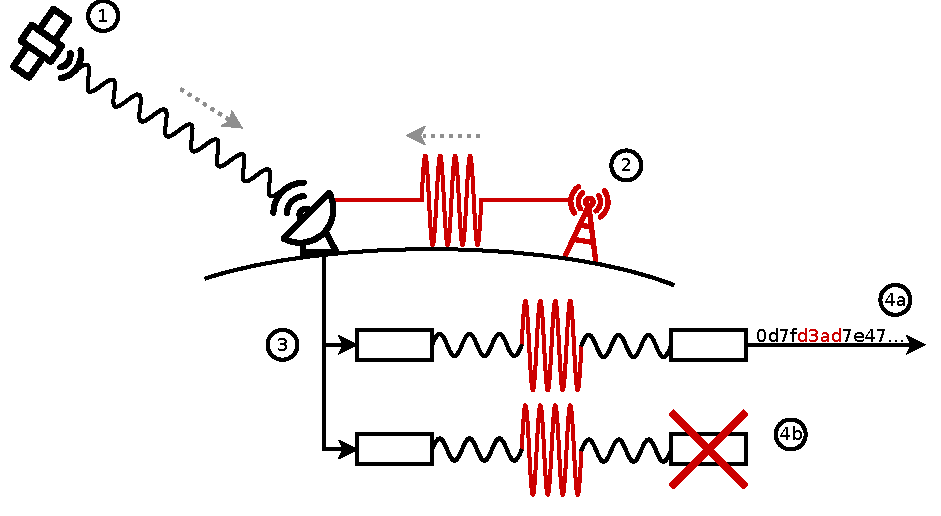
\includegraphics[width=\columnwidth]{diagrams/attack_illustration.pdf}
    \caption{An illustration of the attacks described in this paper. 1)~The satellite broadcasts a signal; 2)~A ground-based attacker injects a crafted signal, overshadowing the legitimate signal; 3a)~The victim receiver decodes the attacker-controlled data, poisoning derived datasets; 3b)~The injected signal exploits vulnerabilities in the protocol decoders, resulting in denial of service or arbitrary code execution.}
    \label{fig:attack-illustration}
\end{figure}

Earth observing satellite systems are widely used in a variety of contexts, providing high-resolution images and sensor readings which update within hours or less of the initial readings being taken.
Accordingly, a growing market for satellite-derived datasets has emerged which derive data for specific purposes including forest fire, dust storm detection, ozone layer depletion, and flooding.
Table~\ref{tab:satellite-derived-datasets} summarises a number of currently available satellite-derived datasets, which are derived from a mixture of self-operated, commercial, and open access satellites.

NASA's \textit{Fire Information and Resource Management System} (FIRMS) is one such use case of satellite-derived data, providing a real-time fire notification service which is used for emergency response, disaster planning, and crisis analysis by the fire agencies of over 90 countries. \textbf{TODO: must cite}
FIRMS depends on data derived from the Earth Observing System (EOS) fleet to produce the calibrated images of the Earth's surface overlaid with detected fires seen in Figure~\ref{fig:bushfire}.
This is possible because certain satellites in the EOS fleet contain instruments such as the \textit{Moderate Resolution Imaging Spectroradiometer} (MODIS), which provide near real time calibrated light readings across frequency bands wider than the visible spectrum.
Primarily, the presence of a fire is indicated by high amplitudes in the infrared bands. \textbf{todo: cite MOD14 technical manual}

Specifically, the MODIS instruments are on board \textit{Terra} and \textit{Aqua}, two EOS fleet satellites.
Thanks to their opposite polar sun-synchronous orbits, Terra and Aqua together image the entire surface of the Earth twice per day.
The data is downlinked to receiver stations across the world in a continuous stream known as \textit{direct broadcast}, or instead as a buffered data dump to a few select locations.
As a result, MODIS data is widely available, both from the central NASA archives \textbf{TODO: link} and from any of the \textbf{TODO: number} alternative receiver stations.

Even though Terra and Aqua were launched in 1999 and 2002 respectively, MODIS-derived datasets continue to see broad usage beyond just forest fires.
For example, derived datasets from the digital archives are frequently used for analysing global events, including diseases that pose serious risks to human health~\cite{valleyFever}.
Such long lifespans are common for Earth observing satellites, which are designed to high specifications and have high upfront costs.

However, over the last few decades, attitudes towards securing the wireless channel in communications systems has changed significantly.
Previously, overshadowing the signal to inject data or deny service would have required a costly and highly specialized setup; since the advent of the software-defined radio, such attacks now only require access to hardware available off-the-shelf.
It is now commonly known that, using this hardware, attackers can leverage overshadowing to manipulate communications or deny service in areas such as mobile internet~\cite{yang2019hiding,erni2021adaptover}, GPS~\cite{tippenhauer2011requirements}, and even electric vehicle charging\textbf{TODO: more examples}.
In these cases, the attacker has been enabled by a lack of robust cryptography in the systems being faced.

% TODO: insert diagram of common space comms protocols
% TODO: find out which other satellites are unencrypted, and especially those which are new and use CCSDS
% Are they generally encrypted above the CCSDS layer?

Many Earth observing satellites face similar issues; these systems were built at a time when robust cryptography was uncommon due to less powerful onboard computers.
Therefore, while it is unsurprising that such systems are not resilient against modern adversaries, it is surprising that safety-critical infrastructure depends upon the resulting data.
These satellites include NASA's Earth Observing Fleet and NOAA's GOES fleet, which provide no cryptographic authenticity guarantees.
They also include satellites which only implement cryptography partially, or which is no longer considered secure, or whose keys have been leaked through a data breach.

% TODO: summary paragraph of these
For example, Korean satellite COMS-1 uses single DES~\cite{lrit-key-dec}, which has lead to its keys being successfully reversed from the satellite data. \textbf{TODO: confirm this is an accurate summary from the blog post, which seems to imply that a server was involved}
Additionally, GEO-KOMPSAT-2A had its keys leaked on the Korea Meteorological Administration website, and to this day remain publicly available~\cite{xrit-rx}.
We should continue to expect that more encrypted satellite communications become publicly decryptable, as once-secure encryption standards and practises cause leaked keys, some of which will be irrevocably baked into the firmware.

%Finally, other satellites only sign or encrypt data at the application layer, rather than at the data link layer.
%Although this protects the data itself against spoofing, attackers may still be able to take advantage of vulnerabilities in the early protocol decoding stages, as we demonstrate against the EOS fleet.
%Although this boils down to better software engineering practises, the currently\textbf{todo: prove it?} fragmented nature of satellite data link level protocols has encouraged satellite operators to roll their own implementations.
%Accordingly, there exist fewer battle-tested implementations, leaving the remainder open for exploitation.
%We justify this claim in Section~\textbf{TODO} through a security audit of NASA's \textit{International Planetary Observation Processing Package} (IPOPP), the primary software distribution for decoding and processing EOS fleet protocols and data.

Going back to FIRMS...

We demonstrate that this issue leads to arbitrary code execution against the decoders used by NASA for the EOS fleet.
We also discuss how FIRMS is a case study of relying upon unencrypted MODIS data
Therefore we can say what an attacker can achieve through it.



Fire management and incident response represents one such use case of the MODIS instrument, which has improved the fire response capability of over 90 countries \textbf{TODO: cite}.
Although fire departments have little reason to run their own direct broadcast groundstations, the application is still time-critical.
Therefore, NASA has invested in the Fire Information for Resource Management System (FIRMS)~\cite{firmsIndex}, which provides near real time active fire data, defined to be within three hours of observation.
Among other services, FIRMS provides a fire notification API which will deliver notifications of new and active fires within a requested region, which is used to inform firefighters and coordinate their response.
\textbf{TODO: add information on who uses this service, maybe a table. Does Google Maps use this?}
The data is derived from processing the raw Aqua and Terra data with the programs in IPOPP.

However, despite its importance as trusted infrastructure, FIRMS ultimately relies on unencrypted MODIS data which is therefore vulnerable to signal injection.
Through carefully crafting input data to pass any existing integrity checks in the processing pipeline and overshadowing the X-band radio signal, an attacker has the potential to disrupt the fire detection stages of the pipeline, and therefore anyone who relies upon the data.

We proceed to precisely define the nature of the threat in Section~\ref{sec:threat-model}, and describe how an attacker can exploit FIRMS and other processing pipeline stages in Section~\ref{sec:attack}.
We go on to validate the feasibility of the overshadowing approach in Section~\ref{sec:evaluation}, including the capabilities that the attacker requires to be successful.


\begin{figure}
    \centering
    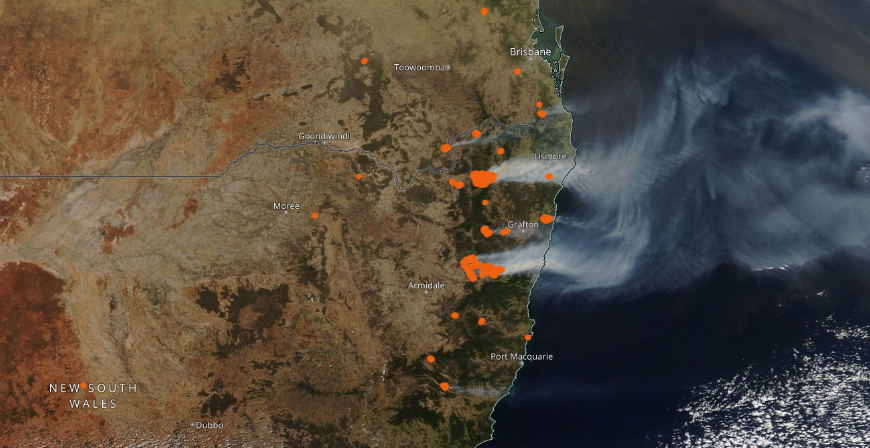
\includegraphics[width=\columnwidth]{diagrams/bushfire.png}
    \caption{The 2019 Australia bushfires as seen from Aqua's MODIS instrument, annotated with the \textit{Fires and Thermal Anomalies} dataset on NASA's worldview.\protect\footnotemark}
    \label{fig:bushfire}
\end{figure}

\footnotetext{Image taken from \url{https://worldview.earthdata.nasa.gov/?v=138.5214305912576,-37.663755528187544,165.90196079866635,-23.47436617591061\&as=2019-09-07-T00\%3A00\%3A00Z\&ae=2019-10-26-T16\%3A00\%3A00Z\&l=MODIS\_Combined\_Thermal\_Anomalies\_All,VIIRS\_SNPP\_Thermal\_Anomalies\_375m\_Day(hidden),VIIRS\_SNPP\_Thermal\_Anomalies\_375m\_Night(hidden),Reference\_Labels\_15m,Reference\_Features\_15m,Coastlines\_15m,VIIRS\_SNPP\_CorrectedReflectance\_TrueColor(hidden),MODIS\_Aqua\_CorrectedReflectance\_TrueColor,MODIS\_Terra\_CorrectedReflectance\_TrueColor(hidden)\&lg=false\&al=true\&av=3.5\&ab=on\&t=2019-09-07-T02\%3A00\%3A00Z}}


% TODO: add info about Google Maps
\begin{table*}
    \resizebox{\textwidth}{!}{%
    \begin{tabular}{lllll}
        \toprule
                     &       & \multicolumn{2}{c}{Satellites} & \\
        \cmidrule(lr){3-4}
        Organization & Usage & Provider & Nature & Data Access \\
        \midrule
        Planet Labs~\cite{planetProducts} & Various (intelligence, infrastructure, & Planet Labs & Self-operated & Commercial \\
                    & land use, water use) & & & \\
        Global Forest Watch~\cite{gfwMap} & Forest monitoring, carbon use, deforestation & Planet Labs & Commercial & Open access \\
        California Forest Observatory~\cite{cfoMap} & Monitoring forest fires in California & Planet Labs & Commercial & Open access \\
        ESRI~\cite{esriMap} & Land-use and land-cover maps & ESA (Sentinel-2) & Open access & Open access \\
        %Salo Sciences (TODO only bring back if I can say something about "forest restoration monitoring" project) & Conservation, climate monitoring & Planet Labs & Commercial & \\
        Meta~\cite{metaMap} & Population density maps & DigitalGlobe & Commercial & Open access \\
        Cloud to Street~\cite{cloudToStreet} & Flood tracking (disasters and insurance) & NASA (Terra/Aqua) & Open access & Commercial \\
        NCX Basemap~\cite{ncxBasemap} & Timber and carbon value monitoring in the USA & NASA & Open access & Commercial \\
        Upstream Tech HydroForecast~\cite{hydroforecast} & Water flow and weather intelligence & NASA (Terra/Aqua) & Open access & Commercial \\
        NASA FIRMS~\cite{nasaFirms} & Fire detection and management & NASA (EOS) & Self-operated & Open access \\
        \bottomrule
    \end{tabular}
    }
    \caption{Information on a number of satellite-derived datasets, including the satellite providers used to source the data.}
    \label{tab:satellite-derived-datasets}
\end{table*}


\subsection{Related Work}

% TODO: GNSS spoofing - mention in related work?
% https://www.usenix.org/conference/usenixsecurity19/presentation/yang-hojoon\textbf{TODO write}
% 
\begin{itemize}
    \item existing work in signal sniffing/spoofing, ads-b?
    \item existing work in satellite security?
    \item explain how our work is novel and builds on these
\end{itemize}

Our work builds on \textbf{TODO}

Existing work has shown that it is possible to spoof satellite signals, particularly when not encrypted; \textbf{TODO} demonstrates this using the GPS positioning satellites.
By exploiting the unauthenticated nature of the signals it is possible to modify the unauthenticated data; our work builds on this by demonstrating that this is also possible for satellites for which the receiving and broadcasting equipment was previously thought to make such attacks prohibitively expensive.
We also look beyond the payload and look at attacks on the data processing system itself to create novel attacks.

\textbf{TODO something about packet-based broadcast vs continuous broadcast?}

There is also wider work in the security community surrounding signal spoofing and its detection -- for instance, Čapkun et al.\ detect GPS spoofing by observing the physical properties of the signal alongside inspecting downlinked data \textbf{TODO cite SPREE}.
\textbf{TODO more?}
We \textbf{TODO}.


% To go in the attack description:
\begin{comment}
The data is downlinked in almost exactly the same format for both the main data dump and the direct broadcast.
Packets from the MODIS instrument are encapsulated wthin the CCSDS Space Packet Protocol (SPP), which are packed within an unencrypted custom data link protocol known as the \textit{Channel Access Data Unit}, or CADU.
Finally, the CADUs are modulated using \textit{Quadrature Phase Shift Keying} (QPSK) and transmitted on the X-band, centered at 8160\,MHz. \textbf{TODO: is this the same for both DB and TDRSS dump?}

% TODO: is such an in-depth explanation required here?
The raw SPP packet data is known as \textit{Level 0}, and is processed through a chain of programs distributed through the IPOPP framework to generate higher-level satellite-derived datasets.
The other EOS fleet satellites are processed in much the same way.
The Level 0 data is processed into \textit{Level 1}: an easier to use heirarchical data format, optionally geolocated to a subpixel accuracy using timing information, the satellite's orbital parameters, and an accurate model of the Earth's surface.
Level 1 data is processed into a variety of \textit{Level 2} datasets, including fire detection, land surface temperature values, vegetation detection, etc.
Finally, certain Level 3 datasets are produced, which generally consist of composites of the Level 2 data for specific purposes, such as analysing post-fire burned areas.
\end{comment}

% Tasked vs untasked images - aka when you have to ask to point the satellite, vs it just gets everything
